This option allows users to determine the event at the base of the 
building by performing an effective free-field site response 
analysis of a soil column. In this panel the user specifies a ground 
motion at the bottom of the column. After the soil layers have been properly 
defined, the motion at the ground surface are given at the end 
of the analysis and that motion will be used in the 
simulation of the building response. 

\begin{figure}[!htbp]
  \centering {
    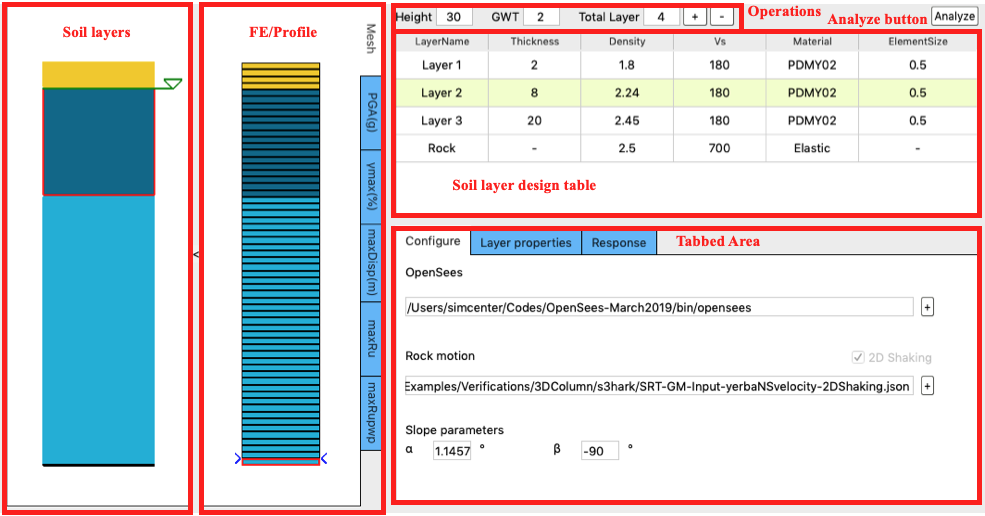
\includegraphics[width=0.8\textwidth]
    {usage/figures/s3hark1.png} }
  \caption{Site Response Analysis Event}
  \label{fig:s3hark1}
\end{figure}

The UI of the Site Response is shown in \Cref{fig:s3hark1}. It is split into the following areas:
\begin{enumerate}
\item Soil Column Graphic: The first graphic on the left of the panel shows a visualization of the soil column.
\item FE Mesh Graphic: The second graphic on the left shows 
the finite element mesh and profile plots. Selecting any of the tabs on the right inside this graphic (i.e, PGA, $\gamma_{max}$, maxDisp, maxRu, maxRuPWP) will show various results
from the simulation at the mesh points.
\item Operations Area: The right side of this area shows some information (e.g., total height and number of soil layers), includes the Ground Water Table (GWT) input field, and plus and minus buttons. If the user presses the plus button, a layer is added below the selected layer. If the minus button is pressed the selected layer is removed. The GWT input field allows the user to specify the level of the ground water table.
\item Soil Layer Table: This table is where the user provides the characteristics of the soil layer, such as layer thickness, density, $V_{s30}$, material type, and element size in the finite element mesh.
\item Tabbed Area: This area contains the three tabbed widgets described below.

\begin{enumerate}
  \item Configure Tab: This tab allows the user to specify the path to the OpenSees executable and to a ground motion file that represent the ground shaking at the bedrock. The rock motion file must follow the SimCenter event format. Examples of SimCenter event files are available with the \href{https://github.com/NHERI-SimCenter/EE-UQ/tree/master/example1/event}{source code}.
  \item Layer Properties Tab: This tab allows the user to enter additional material properties for the selected soil layer (\Cref{fig:s3hark3}).
  \item Response Tab: Once the site response analysis has been performed, this tab provides information about element and nodal time varying respone quantaties.
  \item Run Tab: Opens up a window in which by using the up and down arrows on the keyboard the dino will jump up and down. Something to do if the site response analysis is taking too long, which it may if many soil layers are used.
\end{enumerate}

\item Analyze Button: This button shall be used to run the simulation locally. A progress bar will show the status of the analysis. This allows the user to review the ground motion predicted at the surface.
\end{enumerate}

\begin{figure}[!htbp]
  \centering {
    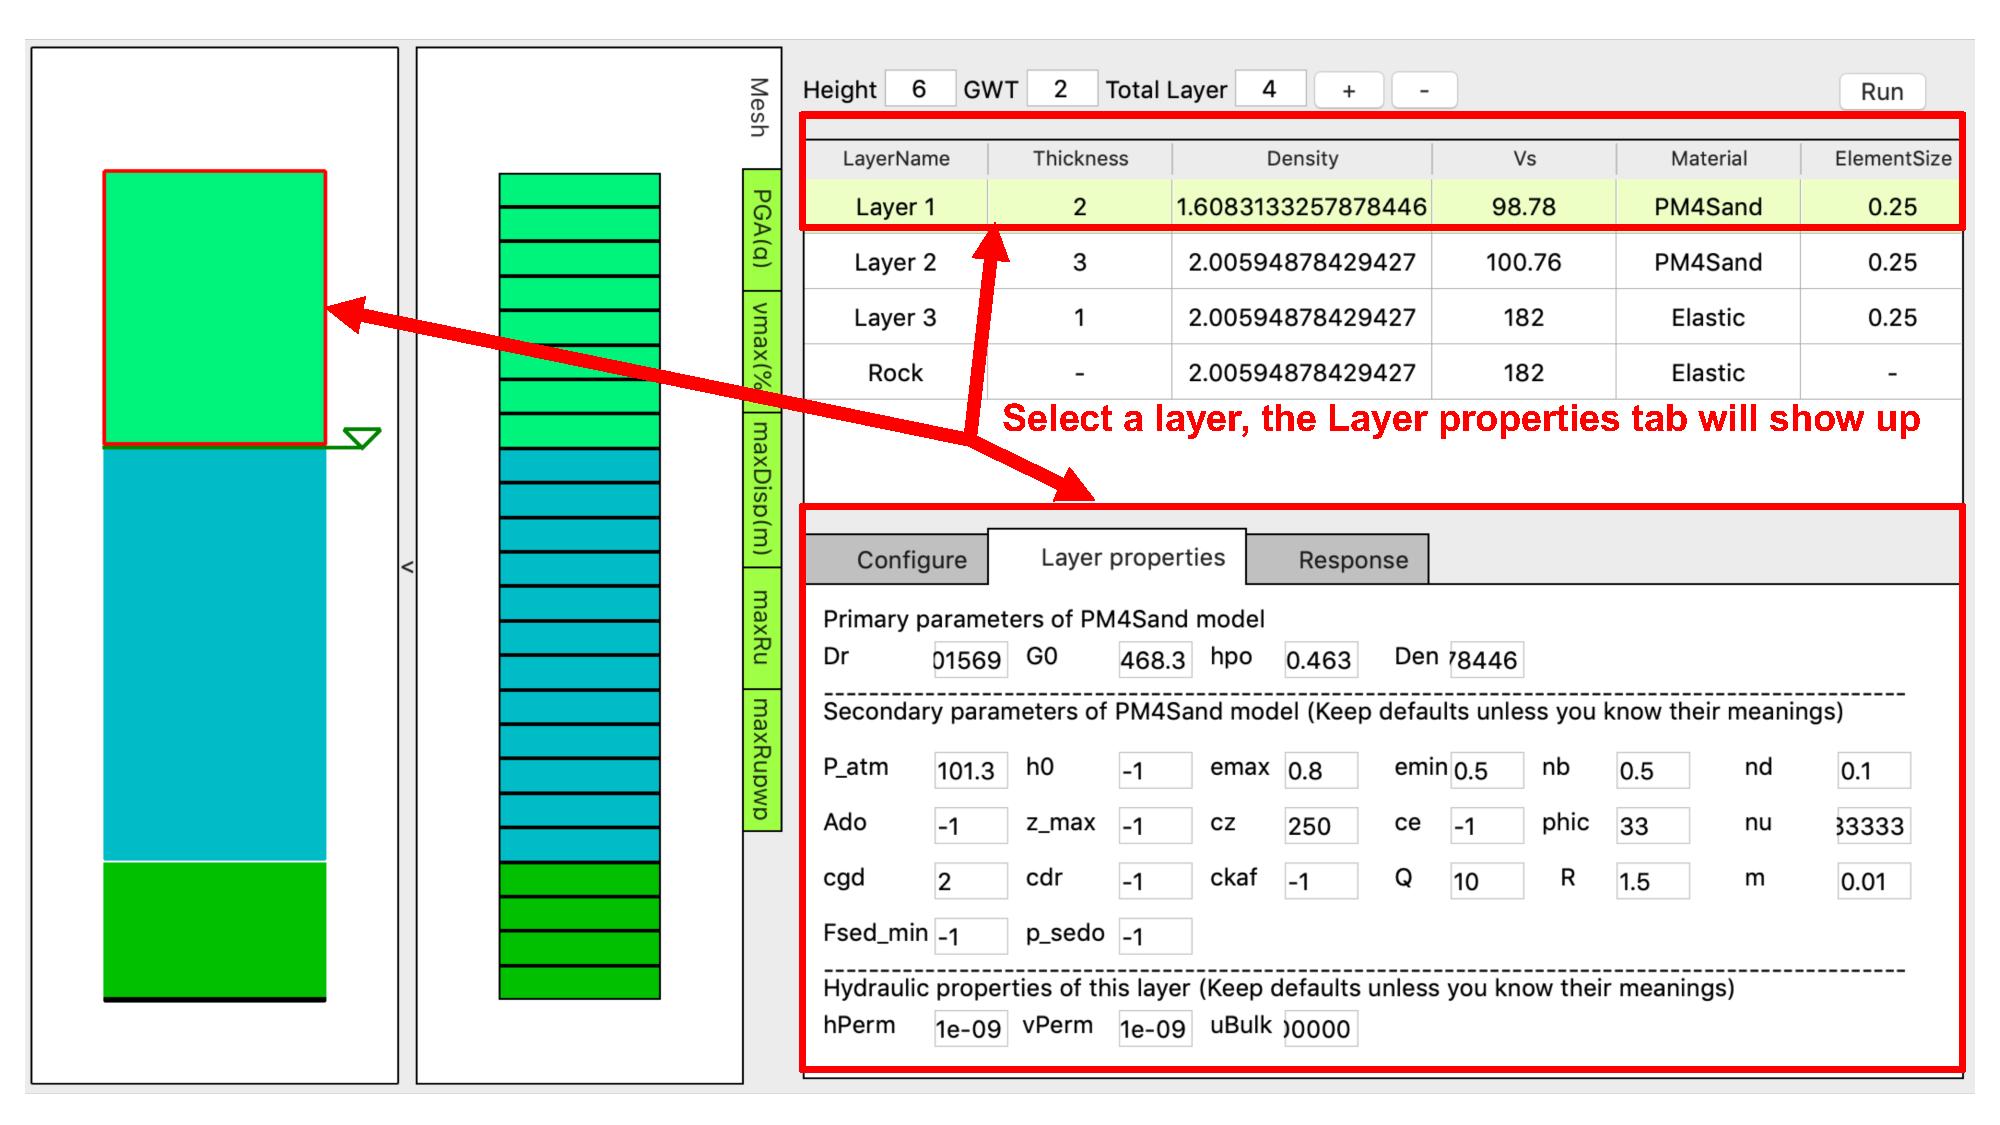
\includegraphics[width=0.8\textwidth]
    {usage/figures/s3hark3.pdf} }
  \caption{Soil Layer Modification in Site Response }
  \label{fig:s3hark3}
\end{figure}

Upon the finish of the finite element analysis, the ground motion at the soil surface (\Cref{fig:s3hark4}) will be stored in EE-UQ's input file.
This computed motion will be applied during the simulation.

\begin{figure}[!htbp]
  \centering {
    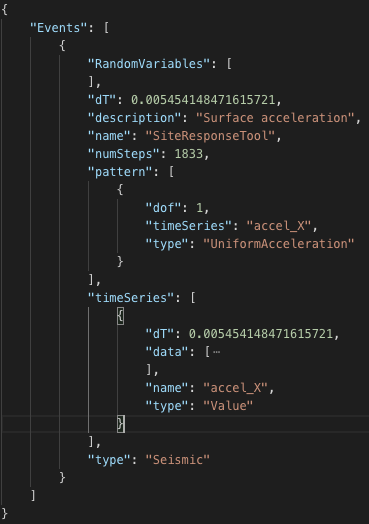
\includegraphics[width=0.4\textwidth]
    {usage/figures/s3hark4.png} }
  \caption{Simulated Motion at the Surface of the Ground}
  \label{fig:s3hark4}
\end{figure}

Random Variables: The current version of the Site Response event type does not support random variables.\\

NOTES: 
\begin{enumerate}
\item Variables are assumed to have m, kPa, and kN units in the Site Response panel.
\item If the Analyze button is not pressed, no simulation will be performed. If no simulation is performed there will be no ground motions provided to the building.
\end{enumerate}
